% This is text associated with the open textbook "Open Electromagnetics"
% See immediately below for author, date
% This work is licensed under the Creative Commons Attribution-ShareAlike 4.0 International License. (CC BY-SA 4.0) 
% To view a copy of the license, visit http://creativecommons.org/licenses/by-sa/4.0/

%ORB TITLE How Antennas Radiate
%ORB AUTHOR 0        # S.W. Ellingson, Virginia Tech (ellingson@vt.edu)
%ORB DATE 20191126   # yyyymmdd
%ORB ABSTRACT 

\label{m0201_How_Antennas_Radiate} % <-- Must match name of this file and module directory name.  Don't mess with this!

An antenna is a \emph{transducer}; 
\index{transducer}
that is, a device which converts signals in one form into another form.
In the case of an antenna, these two forms are (1) conductor-bound voltage and current signals and (2) electromagnetic waves.
Traditional passive antennas are capable of this conversion in either direction.
In this section, we consider the transmit case, in which a conductor-bound signal is converted into a radiating electromagnetic wave.
Radiation from an antenna is due to the time-varying current that is excited by the bound electrical signal applied to the antenna terminals.

{\bf Why ideal transmission lines \emph{don't} radiate.}
To describe the process that allows an antenna to transmit, it is useful to first consider the scenario depicted in Figure~\ref{m0201_fTLonly}.
%
\begin{figure}[b!] % <--- "[b!]" for first figure in section *only*; delete for 2nd and subsequent figures
\begin{center}
\pdftooltip{{  % note double braces
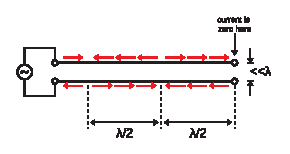
\includegraphics[width=3in]{modules/m0201_fTLonly.eps} 
% https://commons.wikimedia.org/wiki/File:Standing_Wave_Creation.svg
}}{Circuit with sinusoidal source on left connected to two parallel lines ending in open terminal on right. From the open terminal to a distance of lambda over 2 to the left, current on the bottom line moves left and current on the top line moves right. From a distance of lambda over two toward the source, current on the bottom line moves right and current on the top line moves left. To the left of that, current on the bottom line moves left and current on the top line moves right. The distance between the two transmission lines is much less than lambda. 
}
\end{center}
\centerline{\scriptsize 
\copyright~\hyperref[m0201_fTLonly_Credit]{S.\ Lally} 
\href{https://creativecommons.org/licenses/by-sa/4.0/}{CC BY-SA 4.0} 
} % \centerline  
\caption{
\label{m0201_fTLonly}
Twin lead transmission line terminated into an open circuit, giving rise to a standing wave.
}
\end{figure}
%
Here a sinusoidal source is applied to the input of an ideal twin lead 
\label{twin lead}
transmission line.  
The spacing between conductors is much less than a wavelength, and 
the output of the transmission line is terminated into an open circuit.

Without any additional information, we already know two things about the current on this transmission line.
First, we know the current must be identically zero at the end of the transmission line.
Second, we know the current on the two conductors comprising the transmission line must be related as indicated in Figure~\ref{m0201_fTLonly}.
That is, at any given position on the transmission line, the current on each conductor is equal in magnitude and flows in opposite directions.

Further note that Figure~\ref{m0201_fTLonly} depicts only the situation over an interval of one-half of the period of the sinusoidal source.  For the other half-period, the direction of current will be in the direction \emph{opposite} that depicted in Figure~\ref{m0201_fTLonly}.  
In other words: The source is varying periodically, so the sign of the current is changing every half-period.
Generally, time-varying currents give rise to radiation.
Therefore, we should expect the currents depicted in Figure~\ref{m0201_fTLonly} might radiate.
We can estimate the radiation from the transmission line by interpreting the current as a collection of Hertzian dipoles.
\index{Hertzian dipole}
For a review of Hertzian dipoles, see Section~\ref{m0197_Radiation_from_a_Hertzian_Dipole}; however, all we need to know to address the present problem is that superposition 
\index{superposition}
applies.  That is, the total radiation is the sum of the radiation from the individual Hertzian dipoles.
Once again looking back at Figure~\ref{m0201_fTLonly}, note that each Hertzian dipole representing current on one conductor has an associated Hertzian dipole representing the current on the other conductor, and is only a tiny fraction of a wavelength distant.   Furthermore, these pairs of Hertzian dipoles are identical in magnitude but opposite in sign.
Therefore, the radiated field from any such pair of Hertzian dipoles is approximately zero at distances sufficiently far from the transmission line.
Continuing to sum all such pairs of Hertzian dipoles, the radiated field remains approximately zero at distances sufficiently far from the transmission line.
We come to the following remarkable conclusion:
%
%%%%%%%%%%%%%%%%%%%%%%%%%%%%%%%%%%%%%%%%%%%%%%%
%ORB HIGHLIGHT
\begin{mdframed}[backgroundcolor=yellow!20,nobreak=true] 
The radiation from an ideal twin lead transmission line with open circuit termination is negligible at distances much greater than the separation between the conductors.
\end{mdframed}
%%%%%%%%%%%%%%%%%%%%%%%%%%%%%%%%%%%%%%%%%%%%%%%
%
Before proceeding, let us be clear about one thing: 
The situation at distances which are \emph{not} large relative to separation between the conductors is quite different. 
This is because the Hertzian dipole pairs do not appear to be quite so precisely collocated at field points close to the transmission line.  
Subsequently the cancellation of fields from Hertzian dipole pairs is less precise.
The resulting sum fields are not negligible and depend on the separation between the conductors.  
For the present discussion, it suffices to restrict our attention to the simpler ``far field'' 
\index{far field}
case.

{\bf A simple antenna formed by modifying twin lead transmission line.}
Let us now consider a modification to the previous scenario, shown in Figure~\ref{m0201_fTLESD}.
%
\begin{figure}[b!] % <--- "[b!]" for first figure in section *only*; delete for 2nd and subsequent figures
\begin{center}
\pdftooltip{{  % note double braces
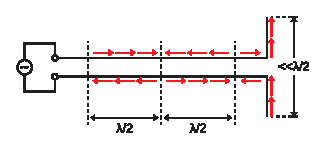
\includegraphics[width=3in]{modules/m0201_fTLESD.eps} 
% https://commons.wikimedia.org/wiki/File:Electrically-Short_Dipole.svg
}}{Circuit with sinusoidal source on left connected to two parallel lines ending in open terminal on right. From the open terminal to a distance of lambda over 2 to the left, current on the bottom line moves left and current on the top line moves right. From a distance of lambda over two toward the source, current on the bottom line moves right and current on the top line moves left. To the left of that, current on the bottom line moves left and current on the top line moves right. The distance between the two transmission lines is much less than lambda. The lines connect to 2 short pieces of wire at a 90 degree angle. Currents on these short pieces flows up.  The length from end to end of the resulting antenna is much less than lambda over two.}
\end{center}
\centerline{\scriptsize 
\copyright~\hyperref[m0201_fTLESD_Credit]{S.\ Lally} 
\href{https://creativecommons.org/licenses/by-sa/4.0/}{CC BY-SA 4.0} 
} % \centerline
\caption{
\label{m0201_fTLESD}
End of the twin lead transmission line fashioned into an electrically-short dipole (ESD).
}
\end{figure}
%
In the new scenario, the ends of the twin lead are bent into right angles.
This new section has an overall length which is much less than one-half wavelength.
To determine the current distribution on the modified section, we first note that the current must still be precisely zero at the ends of the conductors, but not necessarily at the point at which they are bent.
Since the modified section is much shorter than one-half wavelength, the current distribution on this section must be very simple.  
In fact, the current distribution must be that of the electrically-short dipole (ESD), exhibiting magnitude which is maximum at the center and decreasing approximately linearly to zero at the ends. (See Section~\ref{m0198_Radiation_from_an_Electrically-Short_Dipole} for a review of the ESD.)
Finally, we note that the current should be continuous at the junction between the unmodified and modified sections.

Having established that the modified section exhibits the current distribution of an ESD, and having previously determined that the unmodified section of transmission line does not radiate, we conclude that this system radiates precisely as an ESD does.  
Note also that we need not interpret the ESD portion of the transmission line as a modification of the transmission line: Instead, we may view this system as an unmodified transmission line attached to an antenna, which in this case in an ESD. 

{\bf The general case.}
Although we developed this insight for the ESD specifically, the principle applies generally.
That is, any antenna -- not just dipoles -- can be viewed as a structure that can support a current distribution that radiates.
Elaborating:
%
%%%%%%%%%%%%%%%%%%%%%%%%%%%%%%%%%%%%%%%%%%%%%%%
%ORB HIGHLIGHT
\begin{mdframed}[backgroundcolor=yellow!20,nobreak=true] 
A transmitting antenna is a device that, when driven by an appropriate source, supports a time-varying distribution of current resulting in an electromagnetic wave that radiates away from the device.
\end{mdframed}
%%%%%%%%%%%%%%%%%%%%%%%%%%%%%%%%%%%%%%%%%%%%%%%
%
Although this may seem to be simply a restatement of the definition at the beginning of this section -- and it is -- we now see \emph{how} this can happen, and also why transmission lines typically aren't also antennas. 

